\documentclass{article}
\usepackage{graphicx}
\graphicspath{ {Plots/} }
\usepackage[export]{adjustbox}
\usepackage[leftcaption]{sidecap}
\usepackage{amssymb}
\usepackage[utf8]{inputenc}

\title{Statistical Methods in Infectious Disease Modeling}
\date{2017-04-20}
\author{Kaitlyn Stocker}

\begin{document}

\maketitle
\pagenumbering{gobble}
\newpage
\pagenumbering{arabic}
\tableofcontents
\newpage
%notes: 
%-write a 3 sentence (short) intro for each section
%- add references asap
%- convert all simulated examples to the same example - use measles the whole way

\section{Introduction}
%should include general info about infectious disease, general info about statistical inference (overview of MLE and Bayes

\section{Modeling and Inference for Infectious Disease}
\subsection{Deterministic Models} %talk about die-outs, endemic equilibrium, etc... needs work
I began my study of infectious disease modeling by working with a deterministic, continuous time model of an SIR disease. For the sake of simplicity, I began by looking at a closed population in which there was no effect of demographics or migration on the population. 

When modeling the spread of an infectious disease through a population, there are two key parameters of interest: the transmission rate $\beta$, and the recovery rate $\gamma$. The transmission rate is the product of the rate of contact between susceptibles and infecteds in a given population, and the duration of the infection is the average length of time an individual will remain in the infected class. The duration of the infection is then given by the reciprocal of the recovery rate, $frac{1}{\gamma}$. These parameters, together with the initial values of S, I, and R, are the necessary pieces of information required to simulate the spread of the infection through a population. 

The proportion of susceptibles, infecteds, and recovered individuals over time is represented by a series of differential equations given by the following:

\begin{equation}\frac{dS}{dt} = -\beta SI \end{equation}
\begin{equation}\frac{dI}{dt} = \beta SI - \gamma I \end{equation}
\begin{equation}\frac{dR}{dt} = \gamma I \end{equation}

In this model, $\beta SI$ is the transmission term, and represents the number of individuals flowing from the susceptible class into the infected class, and $\gamma I$ represents the flow of individuals from the infected class into the recovered class. 

\paragraph{Simulation}
To produce an example of what this model looks like in action, I simulated the spread of influenza through a boy's boarding school. I took the values of the parameters and the initial conditions from the book **INSERT CITATION**. In this example, $\beta$ is 1.66, and $\gamma$ is $\frac{1}{2.2}$. In a population of 763 boys, at the start of the epidemic 3 were infected and the rest were in the susceptible class. 

As the differential equations defining the model are not possible to solve explicitly, I used Euler's method to solve the system. In R, I ran the system of equations through Euler's method with a 0.01 time step for a period of 15 days. I outputted a data frame that included the value of S, I, and R for each time step through completion. Figure \ref{fig:SIRndSim} shows a plot of the proportion of each infection class over time. 
 
 \begin{figure}[h]
 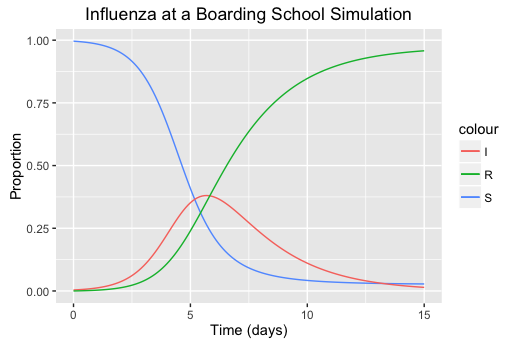
\includegraphics[scale=.5, outer]{SIRndSim.png}
 \caption{Deterministic SIR Simulation}
 \label{fig:SIRndSim}
 \end{figure}

\paragraph{Inference}
I then ran inference on the simulated data to retrieve back the value of $\beta$. To do this, I first created a function that simulated data for a series of $\beta$ values ranging from 0 to 3 with a step of 0.01, maintaining the same initial conditions and $\gamma$ value as the initial simulation. This function created a data frame of results for each value of $\beta$. I then ran a sum of squares function and took the squared difference between the results of my original simulation and the results of my estimation function. A plot of the estimated $\beta$ values against the resulting sum of squares output is presented in figure \ref{fig:SIRndEST}. It is visually evident that the minimum of the function occurs at 1.66, the actual value of $\beta$ that I used to simulate my data. Running the optim function in R to minimize the sum of squares function returned the expected $\beta$ of 1.66. 

\begin{figure}[h]
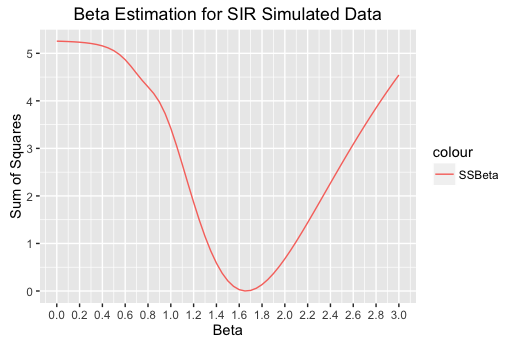
\includegraphics[scale=.5, outer]{BetaEstSIRnd.png}
\caption{Plot of estimated $\beta$ values against their sum of squares output}
\label{fig:SIRndEST}
\end{figure}

\subsection{Stochastic Models}
Deterministic models are useful tools for understanding the interplay of various parameters on the spread of a disease through a population, but they do not account for the inherent randomness of the real world. In reality, the amount of individuals who become infected during a given time interval is not fixed, but is rather randomly distributed. Therefore, the next step in modeling infectious diseases is to add stochasticity to the model. 

\subsubsection{Chain Binomial}
One way of adding stochasticity is to use a chain binomial model. In this type of model, we allow the the number of infecteds at each time step to follow a random binomial distribution in which the number of trials is equal to the number of susceptibles at the previous time step (the pool of individuals who could potentially be infected). If we consider \textit{p} to be the probability that contact occurs between a susceptible and a single infected individual and that the contact results in the infection, then the probability of an individual escaping infection from one infected is given by (1-\textit{p}). In order for a given susceptible to escape infection entirely, they must avoid infection from all infecteds in the population at that time. In this way, the probability of a susceptible escaping infection entirely is given by $(1-p)^{I}$. In this case, the probability that a given susceptible will become infected in a given time step is given by $1-(1-p)^{I}$. It follows that the number of infecteds in a given time step follows a binomial distribution with $S_{t-1}$ as the number of trials and $1-(1-p)^{I}$ as the probability of success. 

The next logical step is to define \textit{p} in terms of our parameters, $\beta$ and $\gamma$. We can do this by defining the probability that a given susceptible will become infected in a given time step (with $I_{t}$ infecteds) as $1-exp(-\beta I_{t}/N)$, where \textit{N} is the total population size. I divided the number of infecteds by the population size to obtain the proportion of infecteds in the population. This was necessary because $\beta$ is derived for use with population proportions, and in this model S, I, and R will refer to the number of individuals in each class. We allow length of the infectious period, $\gamma$, to be equal to the time step. In this way, at the end of each time step the infecteds from the previous time step all move into the recovered class. 

\paragraph{Simulation}

I simulated an SIR infection using the chain binomial model. For consistency and comparison, I used the parameters and starting conditions from the Influenza at a Boarding School example, the same example that I used to simulate the deterministic example, taken from \cite{keeling2011modeling}. 

\begin{figure}[htbp]
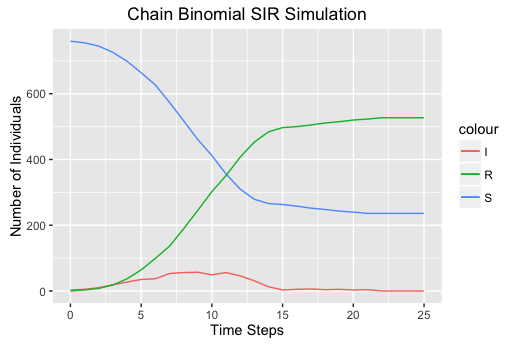
\includegraphics[scale=.5, center]{ChainBinomSim.png}
\caption{Chain Binomial Simulation of Influenza at a Boarding School Example}
\label{fig:ChainBinomSim}
\end{figure}

To achieve the output in figure \ref{fig:ChainBinomSim}, I ran equations (4) through (6) through a loop for 25 time steps. I chose 25 time steps based on the length of the epidemic observed from running the example using a deterministic model. 

\begin{equation} 
I_{t+1} \sim Binomial(S_{t}, 1-exp(\frac{-\beta I}{N})) 
\end{equation}
\begin{equation} 
S_{t+1} = S_{t} - I_{t+1} 
\end{equation}
\begin{equation}
R_{t+1} = R_{t} + I_{t}
\end{equation}

It is clear from figure \ref{fig:ChainBinomSim} and figure \ref{fig:SIRndSim} that the chain binomial model does not have as dramatic of a peak as the deterministic model. 

\paragraph{MLE Inference:}
To run inference on the chain binomial model, I used a maximum likelihood estimate (MLE) approach. To do this, I first found the likelihood function for $\beta$, which is given by equations (7) and (8) below. 


\begin{equation}
\mathcal{L}(\beta) =  \prod_{i=1}^n {I_{i-1}\choose S_{I-1}} p^{I_{i}}(1-p)^{S_{i}}
~, ~where ~ p = 1-exp(\frac{-\beta I_{i-1}}{N})
\end{equation}
This can be simplified to:
\begin{equation}
\mathcal{L}(\beta) \propto p^{I_{[i]}}(1-p)^{S_{[i]}}
\end{equation}

I then used the optimize function in R to compute the value of $\beta$ that maximized the log likelihood function, and received a value of 1.73, which is reasonably close to the value I simulated with, $\beta=1.66$. A plot of the likelihood function can be found in figure \ref{fig:ChainBinomMLE}.

\begin{figure}[htbp]
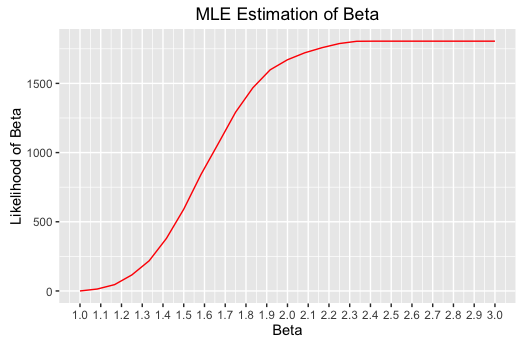
\includegraphics[scale=.5, center]{ChainBinomMLE.png}
\caption{Plot of the likelihood function for $\beta$ for the chain binomial model}
\label{fig:ChainBinomMLE}
\end{figure}

\paragraph{Bayesian Inference:}


Unlike the classical approach, which treats model parameters as fixed values, Bayesian inference treats model parameters as random variables. The distribution of the parameters is calculated via Bayes' Theorem based on information given via a prior distribution and a likelihood computed based on the data. This final distribution is called the posterior distribution, and it gives all relevant information about the parameters, including point and interval estimates. The posterior distribution is defined more precisely in the equation below:

\begin{figure}[htbp]
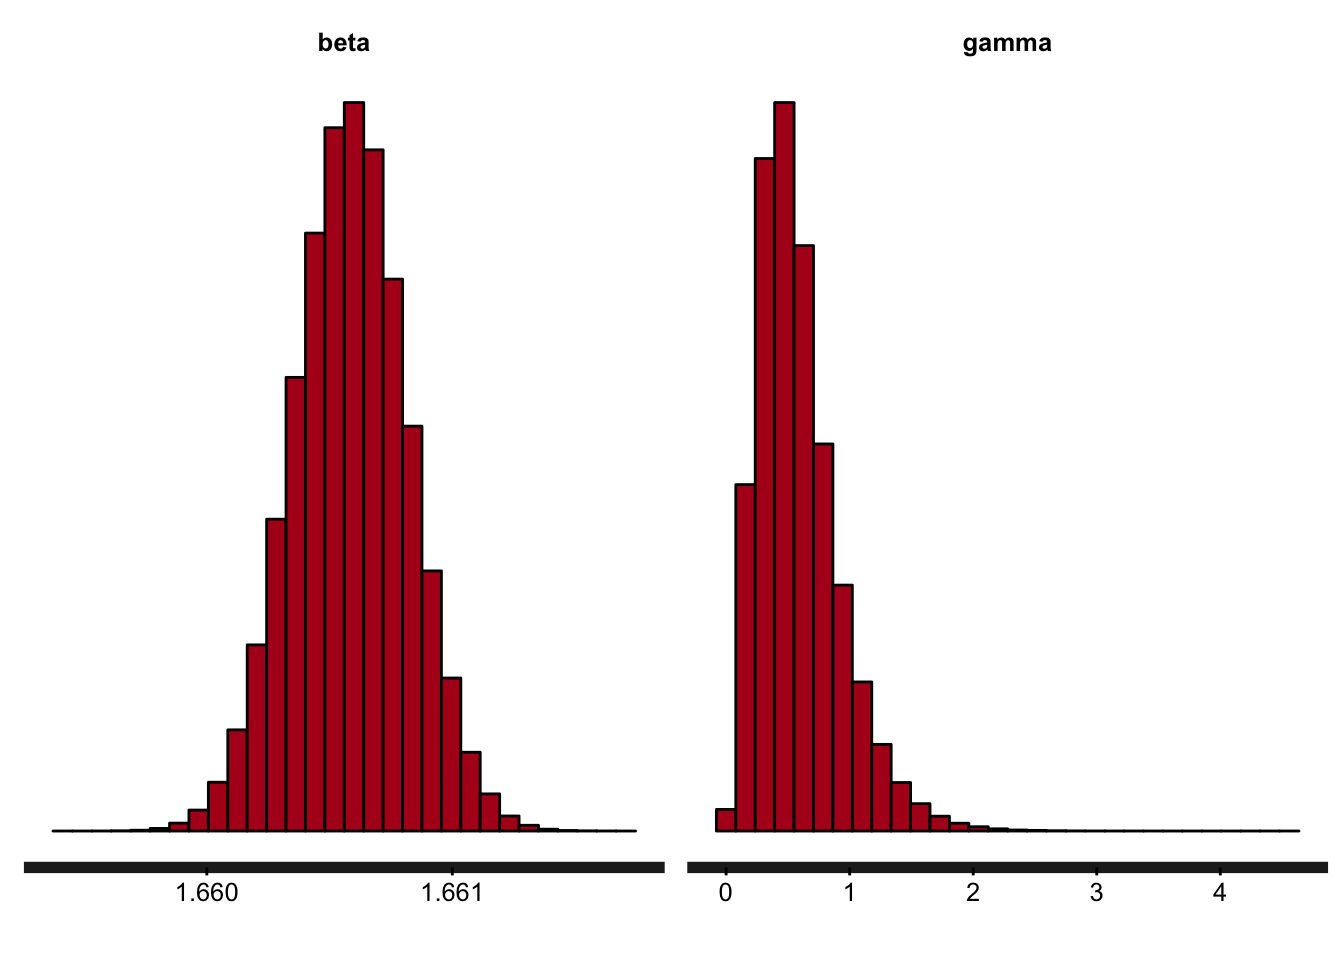
\includegraphics[scale=.25, center]{ChainBinomBayesDensity.png}
\caption{Plot of the posterior density functions for $\beta$ and $\gamma$ respectively}
\label{fig:ChainBinomBayesDensity}
\end{figure}


\begin{figure}[htbp]
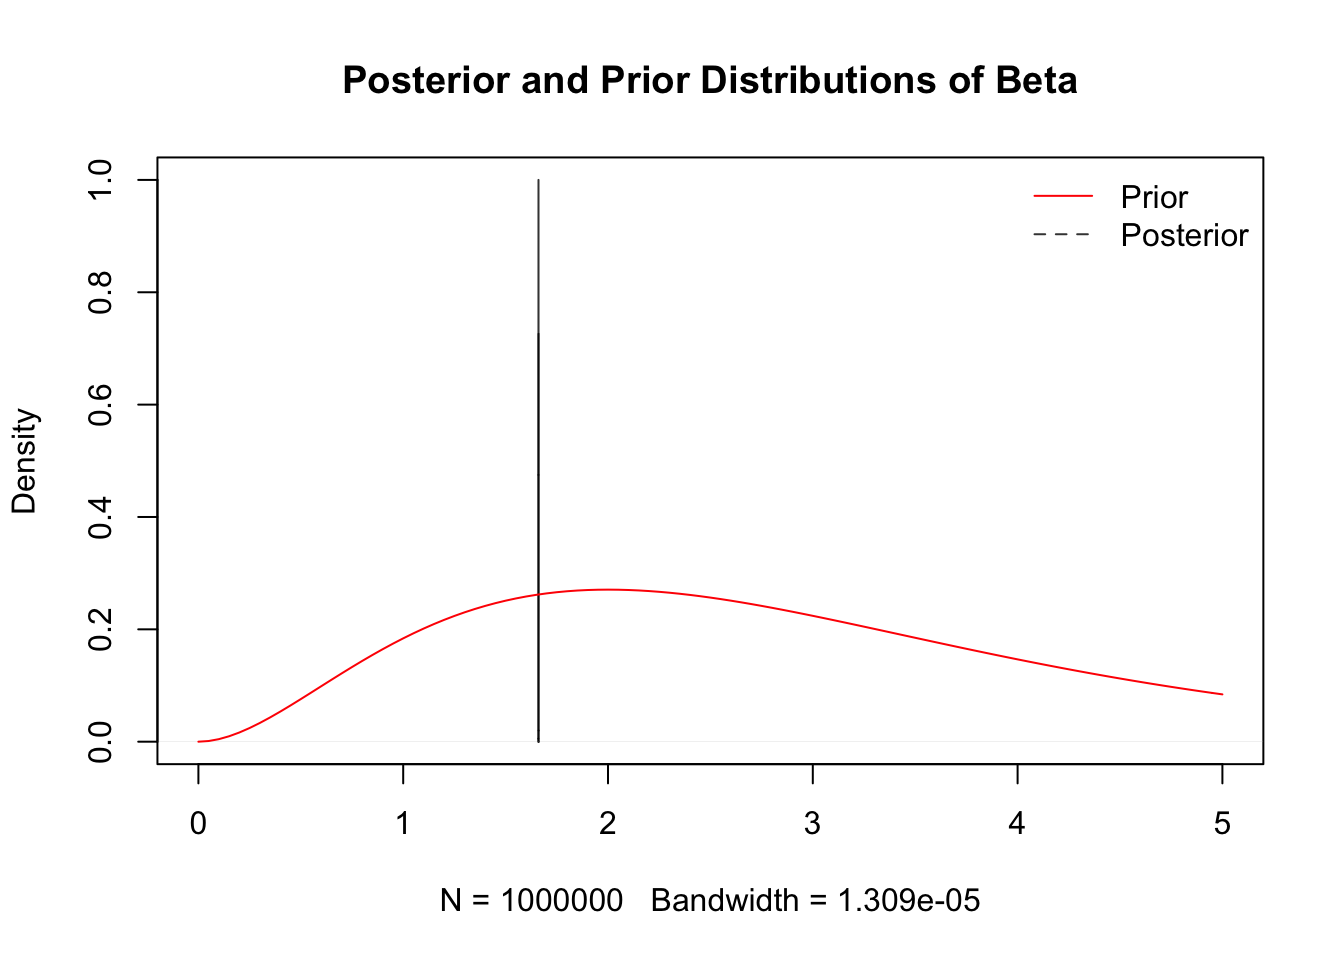
\includegraphics[scale=.2, center]{ChainBinomBetaPosPriorPlot.png}
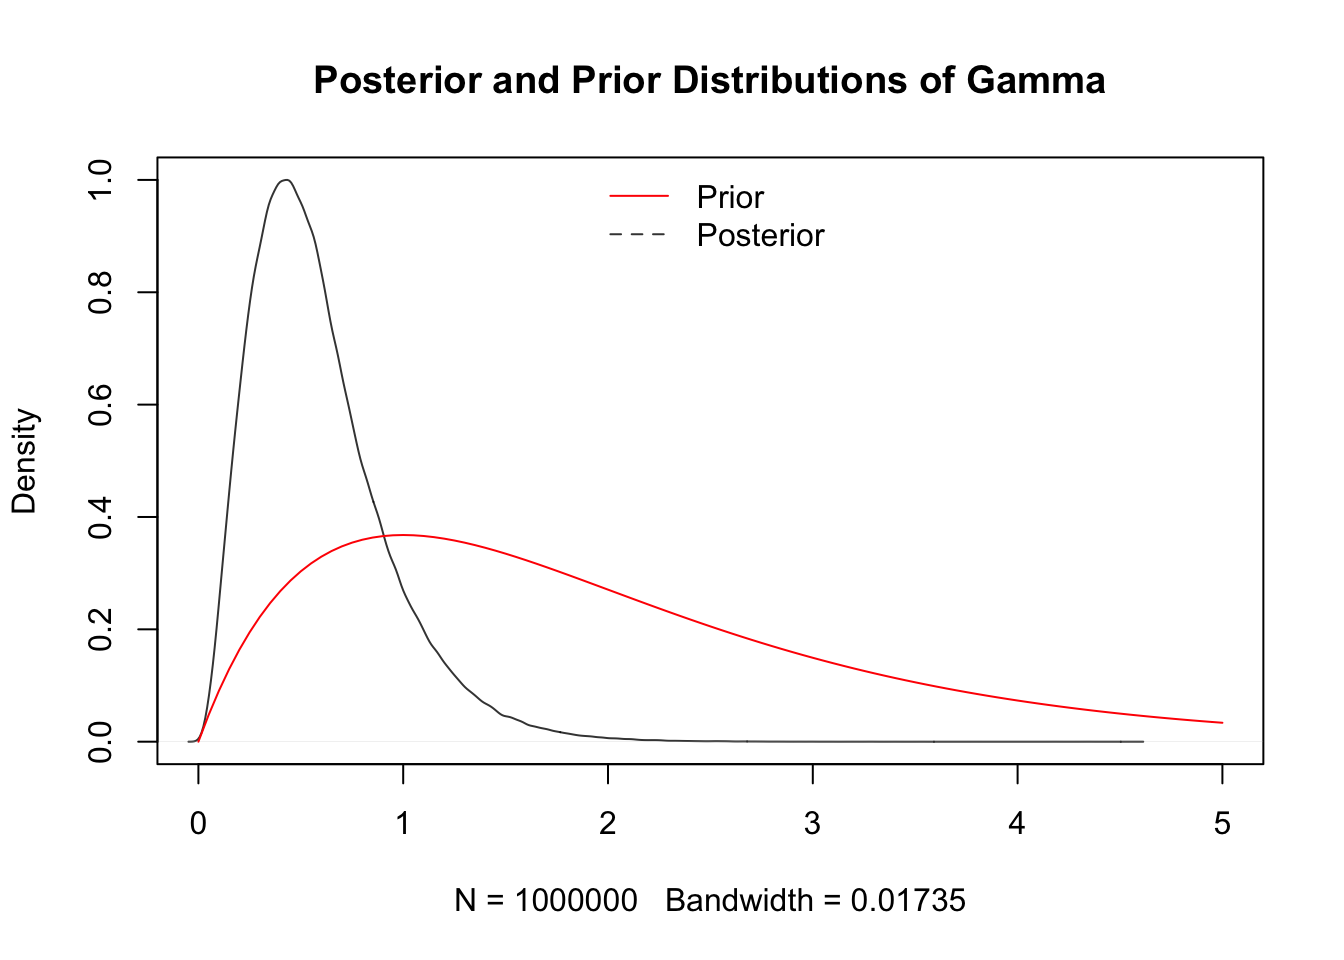
\includegraphics[scale=.2, center]{ChainBinomGammaPosPriorPlot.png}
\caption{Plot of the posterior density function plotted over the prior density function for $\beta$ and $\gamma$ respectively}
\label{fig:ChainBinomPosPriorPlots}
\end{figure}

\begin{equation}
P(\theta \mid y) = \frac{P(\theta)P(y \mid \theta)}{\int P(\theta)P(y \mid \theta) d\theta}
\end{equation}



Where $P(\theta)$ is the prior distribution, $y$ is the data, and $P(y \mid \theta)$ is the likelihood function. 

To run inference on my simulated epidemic data, I used Bayesian inference with the Markov chain Monte Carlo (MCMC) method. The MCMC method allows samples to be drawn from the target distribution - in this case, the samples are drawn from the joint posterior distribution of the model parameter. 

I started by choosing a prior distribution for $\beta$ and $\gamma$. I chose a gamma distribution with shape parameter equal to 3 and scale parameter equal to 1. This distribution has the majority of its density between 0.5 and 5, which is a reasonable range within which to expect $\beta$. For the prior on $\gamma$ I chose a gamma distribution with shape parameter equal to 2 and a scale parameter equal to 1. I chose this prior for $\gamma$ because it has a strong right skew, and $\gamma$ is typically less than one, as it is the reciprocal of the infectious period. 

I used the package RStan to run Bayesian inference with the MCMC method on my simulated chain binomial model, with the aforementioned priors. Figure \ref{fig:ChainBinomBayesDensity} displays the posterior density plots of $\beta$ and $\gamma$. 


The outputted estimate for $\beta$ was 1.66, with a standard error of 0. Recall that the true value of $\beta$ is 1.66. This level of accuracy is possible only with data simulated without any noise. Figure \ref{fig:ChainBinomPosPriorPlots} also shows the lack of error in the posterior density of $\beta$. The outputted estimate for $\gamma$ was 0.76 with a standard error of 0.33. The 95\% credible interval for $\gamma$ was (0.13, 1.40), which contains the true $\gamma$ of $\frac{1}{2.2}$ or 0.455. 

Based on simulated examples, recovery of $\beta$ appears to be more precise than that of $\gamma$. This may, however, be a result of simulation mechanics. For small population sizes, recovery of $\gamma$ was unreliable. However, population size did not affect the ability to accurately recover $\beta$.  

\subsubsection{TSIR}
The TSIR (Time Series Susceptible-Infected Removed) model is a time series, discrete time, stochastic model based on the basic SIR model. It is similar to the chain binomial, although a notable advantage of the TSIR model is that it can be used with reconstructed data. 

Similar to the chain binomial, the time step of the model is set equal to the infectious period ($\frac{1}{\gamma}$). 

The model is defined by the following equations:

\begin{equation}
E(I_{t+1}) = \beta I_{t} S_{t} N^{-1}
\end{equation} 

Where N is the population size, and $I_{t}$ and $S_{t}$ are the number of infected and susceptible individuals at time {\itshape t}, respectively. 

\begin{equation}
I_{t+1} \sim NB(E(I_{t+1}), I_{t})
\end{equation} 

Where NB({\itshape a, b}) indicates the negative binomial distribution with expected value {\itshape a} and clumping parameter {\itshape b}. 
These equations follow the assumption of mass-action transmission with no demographics, as do the previous models specified. 

\paragraph{Simulating}

I simulated epidemic data fit to a TSIR model using the initial conditions and parameters of the influenza example used with previously discussed models. 

In order to allow for estimation of $\gamma$, I made the time step of the simulation an exponentially distributed random variable with $k = \frac{1}{2.2}$. In this way, the expectation of the time step would be equal to 2.2 weeks, the infectious period of influenza. Figure \ref{fig:TSIRsim}. 

\begin{figure}[htbp]
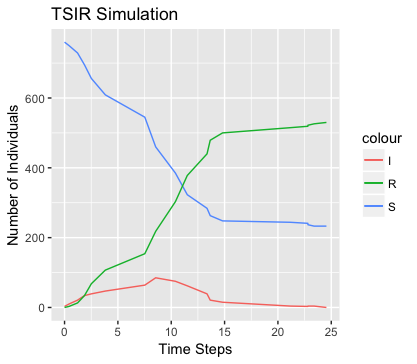
\includegraphics[scale=.5, center]{TSIRSIm.png}
\caption{TSIR simulation of the Influenza at a Boarding School Example}
\label{fig:TSIRsim}
\end{figure}

\subsubsection{Susceptible Reconstruction}
In previous exercises, I had access to perfect and complete simulated data. While having such complete data is convenient, it is not realistic. Data gathered in real-world situations is much less inference-ready than the simulated data I have been using thus far.

Real data deviates from simulated data in a number of significant ways. For one thing, real data is incomplete. Not all cases of a disease are reported, so the number of infecteds at any given time point must be estimated using the number of reported cases multiplied by the reporting rate. There is typically no information about the true number of susceptible or recovered individuals, as collecting this information would be extremely impractical and cost-prohibitive. 

In order to run any kind of meaningful inference on epidemic data, it is necessary to have at minimum the infected and susceptible dynamics over time. Using the reported cases and the rate at which cases are reported, it is easy enough to construct the infected class dynamics. However, reconstructing the susceptible class dynamics is not so straight-forward. 

In order to reconstruct the susceptible class dynamics, let's first define the model. I will continue with the basic SIR model, but this time I am going to add in birth dynamics. The addition of birth dynamics into the susceptible class are crucial to the susceptible reconstruction process. To do this, I will define $B_{t-d}$ as the number of births at time $t-d$. Since infants are born with natural immunity from their mothers, there is a time delay (denoted by $d$) between when a baby is born and when it enters the susceptible class. The length of this delay is dependent on the disease. As before, I define the size of the infected class at a given time point $t$ to be $I_{t}, \in{\{1,...,T\}}$. Similarly, I define the size of the susceptible class at a given time point $t$ to be $S_{t} \in{\{1,...,T\}}$. Equations 12 and 13 give the model specifications. 

\begin{equation}
I_{t} = \beta S_{t-1} I_{t-1}
\end{equation}
\begin{equation}
S_{t} = B_{t-d} + S_{t-1} - I_{t}
\end{equation}

In equation 14 I allow $I_{t}$ to be a product of the number of reported cases, $C_{t}$ and $\rho_{t}$, the reporting rate at time $t$. I define $\rho$ such that when $\rho_{t} =1$, the number of true cases has been fully reported. When $\rho_{t} > 1$, the number of true cases has been underreported. Additionally, I assume that $\rho_{t}$ follows a probability distribution with  $E(\rho_{t}) = \rho$.

\begin{equation}
I_{t} = \rho_{t}C_{t}
\end{equation}

Substituting equation 14 into equation 13, we get: 

\begin{equation}
S_{t} = B_{t-d} + S_{t-1} -  \rho_{t} C_{t}
\end{equation}

If we define $E(S_{t})=\bar{S}$, then we can define a new variable $Z_{t}$ such that $S_{t} = \bar{S} + Z_{t}$, with $E(Z_{t})=0$. In this way, $Z_{t}$ is the deviations from the mean of $S_{t}$. $Z_{t}$ therefore follows the same recursive relationship as $S_{t}$, and can be defined as follows:

\begin{equation}
Z_{t} = B_{t-d} + Z_{t-1} -  \rho_{t} C_{t}
\end{equation}

If we allow $Z_{0}$ to be the initial value of Z, we can rewrite the previous equation to look like the following:

\begin{equation}
Z_{t} = Z_{0} + \sum_{i=1}^{t} B_{i-d} - \sum_{i=1}^{t} \rho_{i}C_{i}
\end{equation}

To de-clutter this notation, allow $Y_{t}=\sum_{i=1}^{t} B_{i-d}$ and $X_{t}= \sum_{i=1}^{t}C_{i}$. Additionally, we will assume a constant reporting rate. Now we can rewrite equation 17 as a simple linear regression equation:

\begin{equation}
Y_{t} = -Z_{0} + Z_{t} + \rho X_{t}
\end{equation}

Thus we have a linear regression equation relating cumulative births ($Y_{t}$) to cumulative reported cases ($X_{t}$). The susceptible dynamics $Z_{t}$ are the regression remainder to equation 18, and can thus be fully reconstructed. 

\paragraph{Simulated Susceptible Reconstruction Example}
In order to validate the accuracy of the susceptible reconstruction method taken from \{citation\}, I first used the method on simulated data. This way, I was able to compare the reconstructed susceptible dynamics to the true, simulated dynamics. 

I first simulated an infection with transmission rate $\beta = 1.66$ and recovery rate $\gamma = 1/2.2$ using the previously defined TSIR model, with one modification. I added birth dynamics to allow the use of susceptible reconstruction. I simulated births using a birth rate of 12 births per 1,000 people annually \{citation\}. 

Following the given method for reconstructing susceptible dynamics, I took the regression remainder from equation 18 and obtained $Z_{t}$. Figure \ref{fig:ZvsS} shows the reconstructed dynamics plotted alongside the true susceptible dynamics. The curves are equivalent, but as per definition $Z_{t}$ is centered around zero. 

\begin{figure}[htbp]
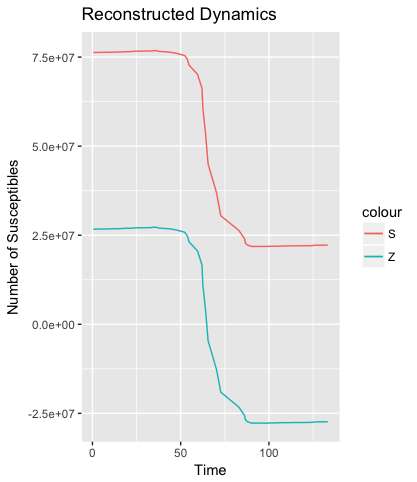
\includegraphics[scale=.5, center]{ZvsSplot.png}
\caption{Comparison of reconstructed susceptible dynamics, $Z$, and the true susceptible dynamics $S$ from the original simulation.}
\label{fig:ZvsS}
\end{figure}

In order to fully reconstruct the susceptible dynamics, it would be necessary to know $\bar{S}$. However, it is not possible to compute the mean number of susceptibles directly, as we are assuming we do not have any data about the true susceptible dynamics. Therefore, I had to instead infer $\bar{S}$ along with the other model parameters ($\beta$ and $\gamma$) when I performed Bayesian Inference. 

I defined the prior on $\bar{S}$ to be normal with a mean of one fifth the initial population size and a standard deviation that was half of the mean. In other words, if we allow $N_{0}$ to be the initial population size, then I defined the prior on $\bar{S}$ as follows: $\bar{S} \sim Normal(\frac{N_{0}}{5}, \frac{N_{0}}{10})$. I then proceeded to replace any instance of $S_{t}$ in the model definition with the equivalent expression $\bar{S} + Z_{t}$. 

After running inference on my reconstructed susceptible dynamics, I took the upper and lower bounds from the $95\%$ Credible Interval of $\bar{S}$ and used those values to obtain upper and lower bounds on the true susceptible dynamics. \ref{fig:SR} shows a plot of the true susceptible dynamics (from the simulation) contained within the upper and lower bounds of the $95\%$ credible interval for the reconstructed dynamics. The true values of $\beta$ and $\gamma$ were also contained within their respective $95\%$ credible intervals. 

\begin{figure}[htbp]
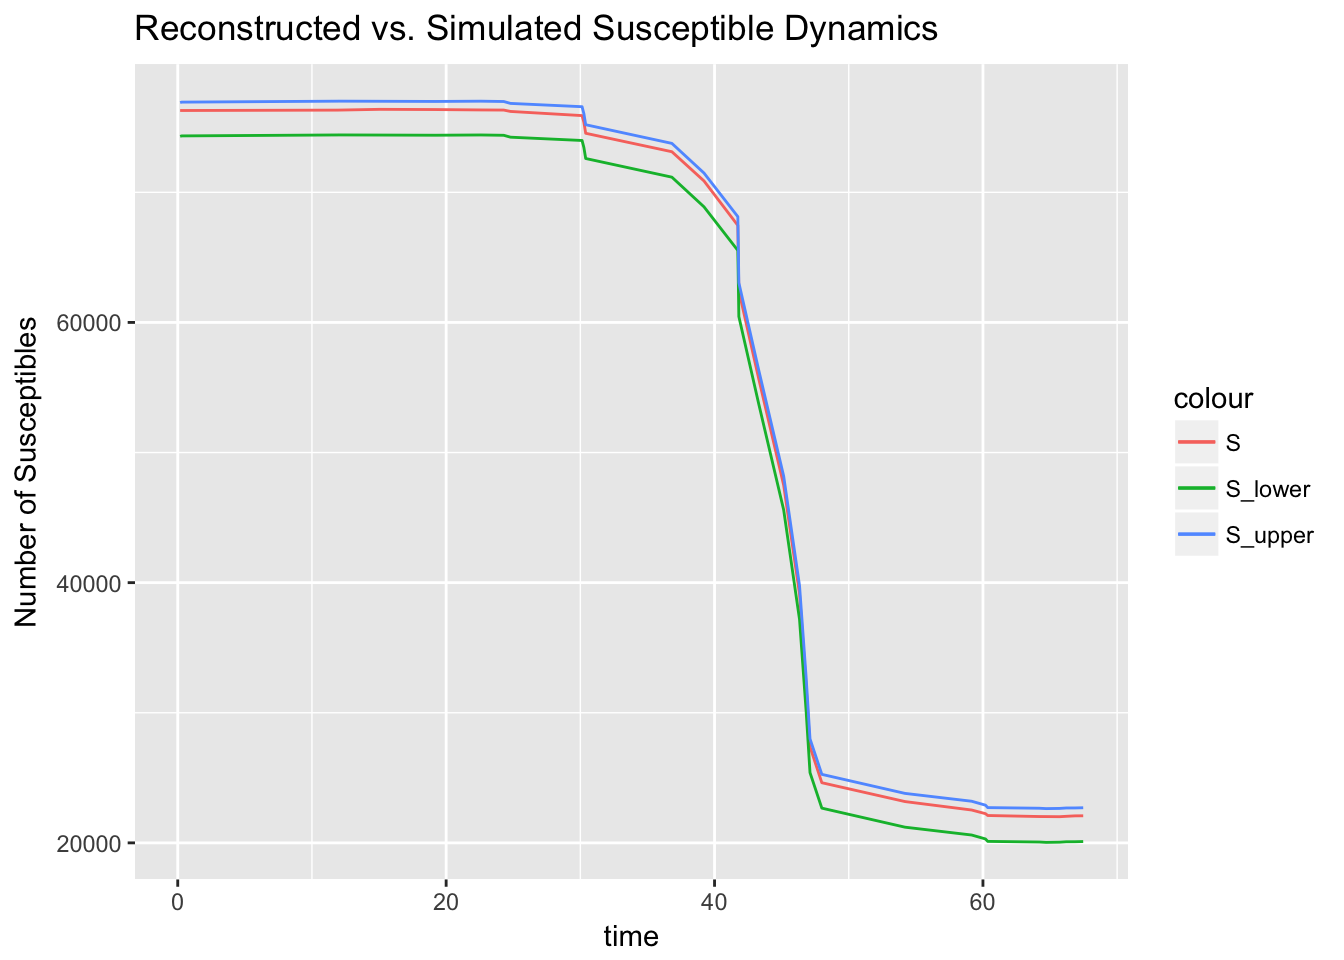
\includegraphics[scale=.25, center]{SRplot.png}
\caption{Plot of the true, simulated susceptible dynamics with the upper and lower estimated susceptible dynamics. The upper and lower bounds were obtained by taking the upper and lower limits of the 95\% credible interval for the mean number of susceptibles, and adding each value to $Z_{t}$. The true number of susceptibles (in red) is clearly contained within the upper and lower bounds of the reconstructed susceptible dynamics.}
\label{fig:SR}
\end{figure}


\subsection{Spatial Models}

\section{Application to Measles}

\section{Results}

\end{document}